% questions.tex —— 2006 年·普通高等学校招生考试·湖北卷文科 · 题目内容片段（无答案）
% 由 tools/generate_projects.py 依来源总账自 2006/2006_数学真题_湖北文_试题.md 生成，勿手改（改源 MD 后重跑）


\begin{gktip}
\textbf{来源边界}：题签依据固定 PDF 首页照录。题面按固定 PDF 第1–2页转录，印刷页码为296–297。固定副本的发布者、出版者、版次、来源链及官方身份均未核；\texttt{ready} 仅为来源清单中的文件状态，不代表来源认证。固定 PDF 可见范围未见答案、解析或评分。
\end{gktip}

\gkpart{一、选择题}

\begin{question}
\gkti{1}集合 $P=\{x\mid x^2-16<0\}$，$Q=\{x\mid x=2n,\ n\in\mathbb Z\}$，则 $P\cap Q=$\mbox{（　　）}。

（A）$\{-2,\ 2\}$　　（B）$\{-2,\ 2,\ -4,\ 4\}$

（C）$\{-2,\ 0,\ 2\}$　　（D）$\{-2,\ 2,\ 0,\ -4,\ 4\}$

\end{question}
\begin{question}
\gkti{2}已知非零向量 $\vec a,\vec b$，若 $\vec a+2\vec b$ 与 $\vec a-2\vec b$ 互相垂直，则 $\dfrac{|\vec a|}{|\vec b|}=$\mbox{（　　）}。

（A）$\dfrac14$　　（B）$4$　　（C）$\dfrac12$　　（D）$2$

\end{question}
\begin{question}
\gkti{3}已知 $\sin 2\alpha=\dfrac23$，$\alpha\in(0,\pi)$，则 $\sin\alpha+\cos\alpha=$\mbox{（　　）}。

（A）$\dfrac{\sqrt{15}}3$　　（B）$-\dfrac{\sqrt{15}}3$　　（C）$\dfrac53$　　（D）$-\dfrac53$

\end{question}
\begin{question}
\gkti{4}在等比数列 $\{a_n\}$ 中，$a_1=1$，$a_{10}=3$，则 $a_2a_3a_4a_5a_6a_7a_8a_9=$\mbox{（　　）}。

（A）$81$　　（B）$27\sqrt[5]{27}$　　（C）$\sqrt3$　　（D）$243$

\end{question}
\begin{question}
\gkti{5}甲：$A_1\text{、}A_2$ 是互斥事件；乙：$A_1\text{、}A_2$ 是对立事件。那么\mbox{（　　）}。

（A）甲是乙的充分条件但不是必要条件

（B）甲是乙的必要条件但不是充分条件

（C）甲是乙的充要条件

（D）甲既不是乙的充分条件，也不是乙的必要条件

\end{question}
\begin{question}
\gkti{6}关于直线 $m,n$ 与平面 $\alpha,\beta$，有以下四个命题：

① 若 $m\parallel\alpha$，$n\parallel\beta$ 且 $\alpha\parallel\beta$，则 $m\parallel n$；

② 若 $m\perp\alpha$，$n\perp\beta$ 且 $\alpha\perp\beta$，则 $m\perp n$；

③ 若 $m\perp\alpha$，$n\parallel\beta$ 且 $\alpha\parallel\beta$，则 $m\perp n$；

④ 若 $m\parallel\alpha$，$n\perp\beta$ 且 $\alpha\perp\beta$，则 $m\parallel n$。

其中真命题的序号是\mbox{（　　）}。

（A）①②　　（B）③④　　（C）①④　　（D）②③

\end{question}
\begin{question}
\gkti{7}设 $f(x)=\lg\dfrac{2+x}{2-x}$，则 $f\left(\dfrac{x}{2}\right)+f\left(\dfrac{2}{x}\right)$ 的定义域为\mbox{（　　）}。

（A）$(-4,0)\cup(0,4)$　　（B）$(-4,-1)\cup(1,4)$

（C）$(-2,-1)\cup(1,2)$　　（D）$(-4,-2)\cup(2,4)$

\end{question}
\begin{question}
\gkti{8}在 $\left(\sqrt{x}-\dfrac{1}{\sqrt[3]{x}}\right)^{24}$ 的展开式中，$x$ 的幂的指数是整数的项共有\mbox{（　　）}。

（A）3项　　（B）4项　　（C）5项　　（D）9项

\end{question}
\begin{question}
\gkti{9}设过点 $P(x,y)$ 的直线分别与 $x$ 轴的正半轴和 $y$ 轴的正半轴交于 $A,B$ 两点，点 $Q$ 与点 $P$ 关于 $y$ 轴对称，$O$ 为坐标原点，若 $\overrightarrow{BP}=2\overrightarrow{PA}$ 且 $\overrightarrow{OQ}\cdot\overrightarrow{AB}=1$，则点 $P$ 的轨迹方程是\mbox{（　　）}。

（A）$3x^2+\dfrac32y^2=1\ (x>0,\ y>0)$　　（B）$3x^2-\dfrac32y^2=1\ (x>0,\ y>0)$

（C）$\dfrac32x^2-3y^2=1\ (x>0,\ y>0)$　　（D）$\dfrac32x^2+3y^2=1\ (x>0,\ y>0)$

\end{question}
\begin{question}
\gkti{10}关于 $x$ 的方程 $(x^2-1)^2-|x^2-1|+k=0$，给出下列四个命题：

① 存在实数 $k$，使得方程恰有2个不同的实根；

② 存在实数 $k$，使得方程恰有4个不同的实根；

③ 存在实数 $k$，使得方程恰有5个不同的实根；

④ 存在实数 $k$，使得方程恰有8个不同的实根。

其中假命题的个数是\mbox{（　　）}。

（A）0　　（B）1　　（C）2　　（D）3

\end{question}
\gkpart{二、填空题}

\begin{question}
\gkti{11}在 $\triangle ABC$ 中，已知 $a=\dfrac{4\sqrt3}{3}$，$b=4$，$A=30^\circ$，则 $\sin B=$\gkblank{}。

\end{question}
\begin{question}
\gkti{12}接种某疫苗后，出现发热反应的概率为 $0.80$，现有5人接种该疫苗，至少有3人出现发热反应的概率为\gkblank{}。（精确到0.01）

\end{question}
\begin{question}
\gkti{13}若直线 $y=kx+2$ 与圆 $(x-2)^2+(y-3)^2=1$ 有两个不同的交点，则 $k$ 的取值范围是\gkblank{}。

\end{question}
\begin{question}
\gkti{14}安排5名歌手的演出顺序时，要求某名歌手不第一个出场，另一名歌手不最后一个出场，不同排法的总数是\gkblank{}。（用数字作答）

\end{question}
\begin{question}
\gkti{15}半径为 $r$ 的圆的面积 $S(r)=\pi r^2$，周长 $C(r)=2\pi r$，若将 $r$ 看作 $(0,+\infty)$ 上的变量，则 $(\pi r^2)'=2\pi r$ ①，①式可以用语言叙述为：圆的面积函数的导数等于圆的周长函数。对于半径为 $R$ 的球，若将 $R$ 看作 $(0,+\infty)$ 上的变量，请你写出类似于①的式子：\gkblank{}②，②式可以用语言叙述为：\gkblank{}。

\end{question}
\gkpart{三、解答题}

\begin{question}
\gkti{16}设向量 $\vec a=(\sin x,\cos x)$，$\vec b=(\cos x,\cos x)$，$x\in\mathbb R$，函数 $f(x)=\vec a\cdot(\vec a+\vec b)$。

（1） 求函数 $f(x)$ 的最大值与最小正周期；

（2） 求使不等式 $f(x)\geqslant\dfrac32$ 成立的 $x$ 的取值集。

\end{question}
\begin{question}
\gkti{17}某单位最近组织了一次健身活动，活动分为登山组和游泳组，且每个职工至多参加了其中一组。在参加活动的职工中，青年人占 $42.5\%$，中年人占 $47.5\%$，老年人占 $10\%$。登山组的职工占参加活动总人数的 $\dfrac14$，且该组中，青年人占 $50\%$，中年人占 $40\%$，老年人占 $10\%$。为了了解各组不同年龄层次的职工对本次活动的满意程度，现用分层抽样的方法从参加活动的全体职工中抽取一个容量为200的样本。试确定：

（1） 游泳组中，青年人、中年人、老年人分别所占的比例；

（2） 游泳组中，青年人、中年人、老年人分别应抽取的人数。

\Needspace{0.4\textheight}
\end{question}
\begin{question}
\gkti{18}如图，已知正三棱柱 $ABC-A_1B_1C_1$ 的侧棱长和底面边长均为1，$M$ 是底面 $BC$ 边上的中点，$N$ 是侧棱 $CC_1$ 上的点，且 $CN=2C_1N$。
\nopagebreak[4]
\begin{center}% Source: 2006湖北文.pdf, source-relative PDF page 1, Q18.
% Non-scale vector redraw; solid/dashed visibility follows the fixed candidate image.
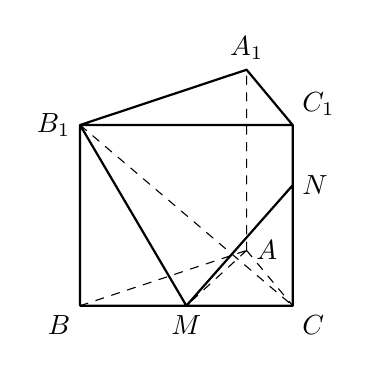
\begin{tikzpicture}[line cap=round,line join=round,x=0.9cm,y=0.9cm]
  \coordinate (B)  at (0,0);
  \coordinate (C)  at (3,0);
  \coordinate (M)  at (1.5,0);
  \coordinate (A)  at (2.35,0.78);
  \coordinate (B1) at (0,2.55);
  \coordinate (C1) at (3,2.55);
  \coordinate (N)  at (3,1.70);
  \coordinate (A1) at (2.35,3.33);

  % Hidden/inner lines visible dashed in the source drawing.
  \draw[dashed] (B)--(A) (A)--(C) (A)--(A1) (B1)--(C) (A)--(M);

  % Prism edges and the two solid segments through M shown in the source.
  \draw[thick] (B)--(C) (B)--(B1) (B1)--(C1) (C)--(C1)
    (B1)--(A1)--(C1) (B1)--(M) (M)--(N);

  \node[below left] at (B) {$B$};
  \node[below] at (M) {$M$};
  \node[below right] at (C) {$C$};
  \node[left] at (B1) {$B_1$};
  \node[above] at (A1) {$A_1$};
  \node[above right] at (C1) {$C_1$};
  \node[right] at (N) {$N$};
  \node[right] at (A) {$A$};
\end{tikzpicture}
\end{center}
\nopagebreak[4]
（1） 求二面角 $B_1-AM-N$ 的平面角的余弦值；

（2） 求点 $B_1$ 到平面 $AMN$ 的距离。

\end{question}
\begin{question}
\gkti{19}设函数 $f(x)=x^3-ax^2+bx+c$ 在 $x=1$ 处取得极值 $-2$，试用 $c$ 表示 $a$ 和 $b$，并求 $f(x)$ 的单调区间。

\end{question}
\begin{question}
\gkti{20}设数列 $\{a_n\}$ 的前 $n$ 项和为 $S_n$，点 $\left(n,\dfrac{S_n}{n}\right)$（$n\in\mathbb N^*$）均在函数 $y=3x-2$ 的图象上。

（1） 求数列 $\{a_n\}$ 的通项公式；

（2） 设 $b_n=\dfrac{3}{a_na_{n+1}}$，$T_n$ 是数列 $\{b_n\}$ 的前 $n$ 项和，求使得 $T_n<\dfrac m{20}$ 对所有 $n\in\mathbb N^*$ 都成立的最小正整数 $m$。

\end{question}
\begin{question}
\gkti{21}设 $A,B$ 分别为椭圆 $\dfrac{x^2}{a^2}+\dfrac{y^2}{b^2}=1$（$a,b>0$）的左、右顶点，椭圆长半轴的长等于焦距，且 $x=4$ 为它的右准线。

（1） 求椭圆的方程；

（2） 设 $P$ 为右准线上的不同于点 $(4,0)$ 的任意一点，若直线 $AP,BP$ 分别与椭圆相交于异于 $A,B$ 的点 $M,N$，证明点 $B$ 在以 $MN$ 为直径的圆内。

\end{question}